\chapter{Introduzione}

Expiration Date è un'applicazione nata per permettere la gestione completa di tutto ciò che riguarda i prodotti alimentari; con essa è infatti possibile gestire gli aspetti relativi:
\begin{itemize}
  \item alla lista della spesa (prodotti che si desidera acquistare)
  \item alla dispensa (prodotti già posseduti)
  \item alle ricette
\end{itemize}

\begin{figure}[H]
  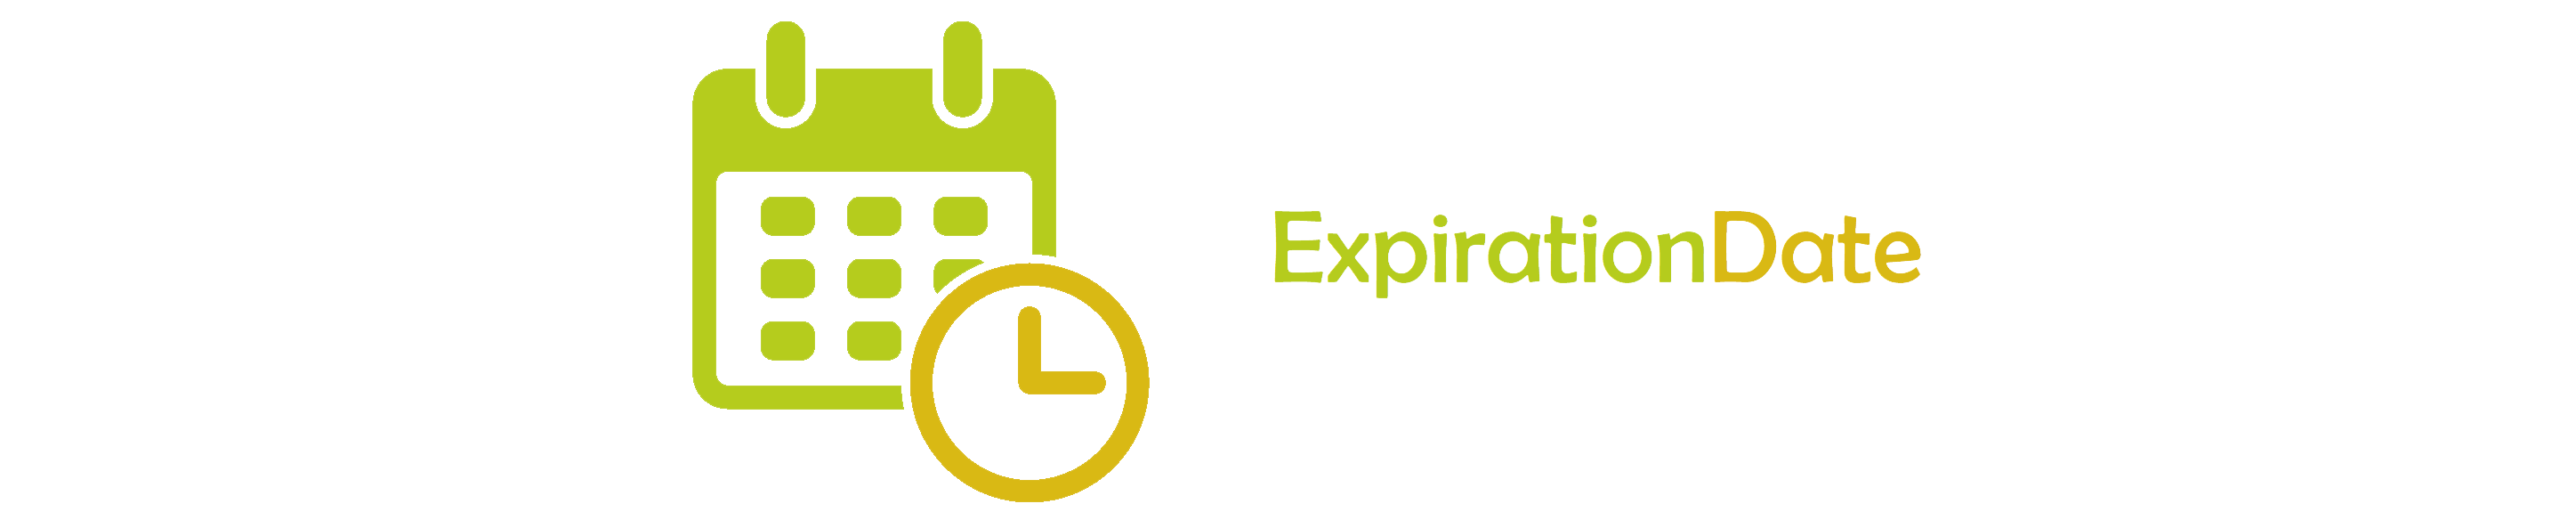
\includegraphics[width=\linewidth]{images/app-logo.png}
  \caption{Logo dell'applicazione.}
  \label{fig:applogo}
\end{figure}

Nel seguito verranno illustrati:
\begin{itemize}
\item i requisiti (funzionali e non funzionali) alla base dello sviluppo dell'applicazione
\item una panoramica generale dell'applicazione, con particolare attenzione all'interfaccia grafica
\item i diagrammi UML (Unified Modeling Language) che descrivono nel dettaglio le funzionalità dell'applicazione e la sua business logic
\item i design patterns implementati, le motivazioni e i vantaggi del loro impiego
\item la tecnica ORM (Object-Relational Mapping) per la gestione della persistenza dei dati e l'interfacciamento con il database
\end{itemize}

Questo elaborato estende l'applicazione sviluppata per l'esame di "Programmazione a oggetti" con l'obiettivo di acquisire nuove competenze nell'ambito dell'inter-operabilità fra programmazione a oggetti e database relazionali. Tramite l'utilizzo di ORM, infatti, ho avuto la possibilità di confrontarmi con un approccio alla gestione dei dati totalmente diverso da quelli visti in precedenza, acquisendo le capacità di: 
\begin{itemize}
\item modellare le entità classiche usate dai database (e definite dal modello relazionale) con un nuovo formalismo, orientato ai linguaggi a oggetti
\item rappresentare le associazioni e il modo con cui le suddette entità interagiscono tra loro attraverso strutture dati tipiche della programmazione (a oggetti ma non solo)
\item integrare concetti tipici della programmazione a oggetti (come l'ereditarietà) in un contesto che nativamente non li prevede
\item accedere a dati memorizzati su database con modalità proprie dei linguaggi di programmazione a oggetti
\item studiare e valutare pregi e difetti di questa metodologia per capirne l'effettiva utilità in un contesto reale, eventualmente confrontandola con altre tecniche (JDBC)
\end{itemize}

Inoltre, rispetto alla versione originale, l'applicazione è stata riprogettata e ha adottato diversi design patterns. In questa fase ho avuto l'opportunità di:
\begin{itemize}
  \item approfondire il concetto di mantenibilità del codice, le best practices per raggiungerla e i suoi vantaggi nel medio e lungo termine
  \item esplorare soluzioni standard a problemi comuni, in modo da poter comunicare efficacemente con esperti del settore
\end{itemize}